

\section{Vérification des facteurs de vue}

\subsection{Méthodologie}

Toutes les études réalisées dans ce chapitre reposent sur la même méthodologie. Les facteurs de vue théoriques sont établis à partir de la Référence~\cite{howell} et sont disponibles en Annexe~\ref{anx:fv}.

Afin d'évaluer quantitativement la qualité des matrices de facteurs de vue obtenues par le code de Monte Carlo Ray Tracing, celles-ci sont comparées à une matrice de référence $F^{\mathrm{ref}}$ via une erreur quadratique moyenne relative (\textit{Relative Root Mean Square Error}, RRMSE). Pour chaque coefficient non négligeable de la matrice de référence, l'erreur relative élémentaire est définie par $\varepsilon_{ij} = (F_{ij}^{\mathrm{calc}} - F_{ij}^{\mathrm{ref}})/F_{ij}^{\mathrm{ref}}$. Afin d'éviter les divisions par des valeurs nulles ou numériquement négligeables, seuls les coefficients vérifiant $\left|F_{ij}^{\mathrm{ref}}\right| > \varepsilon_{\mathrm{th}} = 10^{-15}$ sont retenus dans le calcul, l'ensemble des indices satisfaisant cette condition étant noté $\Omega$. La métrique globale est alors définie comme la racine de la moyenne des carrés des erreurs relatives :

\begin{equation}
\mathrm{RRMSE} = \sqrt{\frac{1}{|\Omega|} \sum_{(i,j)\in \Omega} \varepsilon_{ij}^{2}}.
\label{eq:rrmse}
\end{equation}

Cette grandeur fournit une mesure globale, sans dimension, de l'écart entre la matrice calculée et la matrice de référence : une valeur nulle correspond à une concordance exacte, tandis qu'une augmentation traduit une dégradation progressive de l'accord entre les deux solutions. Le RRMSE est utilisé dans la suite du chapitre pour analyser la convergence et la qualité des résultats pour trois familles de géométries : configurations 3D (Section~\ref{part:verif3D}), 2D (Section~\ref{part:2Dcomp}), et à faces réflectives (Section~\ref{part:verifmiroir}).

\subsection{Résultats}

La vérification du code de lancer de rayons repose sur l'étude de la convergence statistique des facteurs de vue estimés par Monte Carlo. Pour un estimateur non biaisé, le théorème central limite prédit que l'erreur statistique décroît comme $N^{-1/2}$, où $N$ désigne le nombre de rayons simulés. Cette loi constitue la référence attendue pour la convergence de l'erreur.

Trois indicateurs sont suivis au cours des simulations :

\begin{itemize}
    \item la droite de référence de pente $N^{-1/2}$, représentée en noir, qui matérialise le taux de convergence théorique d'un estimateur Monte Carlo ;
    \item la variance moyenne de l'estimateur, représentée en orange, obtenue à partir du moment d'ordre deux des facteurs de vue estimés. Elle caractérise l'incertitude statistique intrinsèque de l'estimation ;
    \item la RRMSE (\emph{Relative Root Mean Square Error}), représentée en bleu, calculée par rapport à la solution de référence. Cet indicateur quantifie simultanément les erreurs statistiques et les éventuelles erreurs numériques liées à la discrétisation géométrique ou à l'algorithme.
\end{itemize}

Les Figures~\ref{fig:verif3D_3D} à~\ref{fig:verifmiroir} présentent l'évolution de ces trois quantités en fonction du nombre de rayons simulés par face pour l'ensemble des cas de validation considérés.

\subsubsection{Simulation MCRT en 3D}
\label{part:verif3D}

\begin{figure}[H]
\centering
\begin{minipage}{0.49\textwidth}
\centering
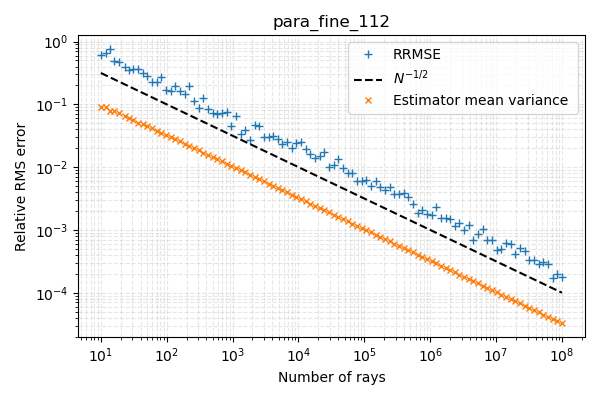
\includegraphics[width=\linewidth]{PICTURES/c2/VERIF/rms_convergence_para_fine_112.png}
\small\textbf{(a) Cas d'un parallélépipède}
\end{minipage}
\hfill
\begin{minipage}{0.49\textwidth}
\centering
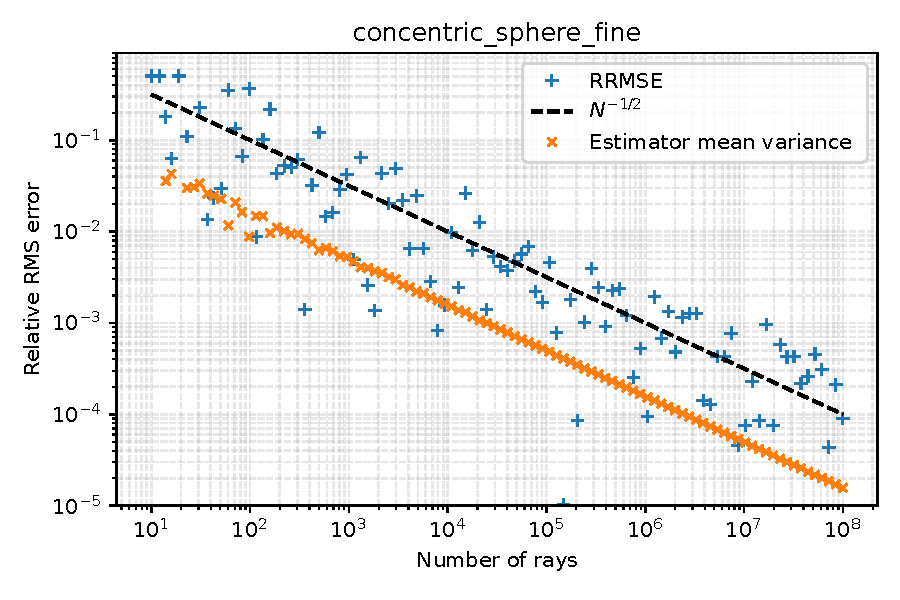
\includegraphics[width=\linewidth]{PICTURES/c2/VERIF/convergence_cs_f.pdf}
\small\textbf{(b) Cas de deux sphères concentriques}
\end{minipage}
\caption{Convergence des facteurs de vue pour deux géométries tridimensionnelles.}
\label{fig:verif3D_3D}
\end{figure}

\subsubsection{Simulation MCRT avec des géométries 2D}
\label{part:2Dcomp}

\begin{figure}[H]
\centering
\begin{minipage}{0.49\textwidth}
\centering
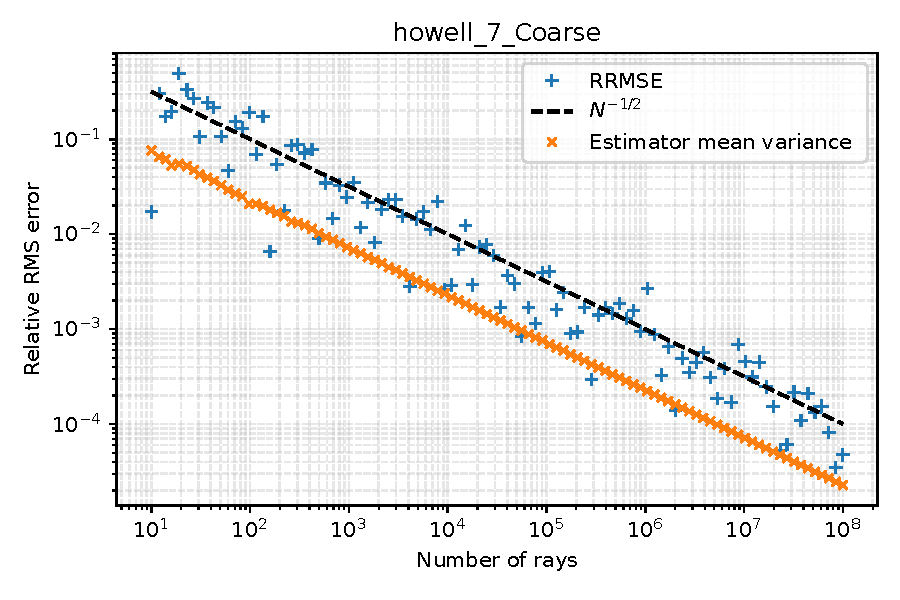
\includegraphics[width=\linewidth]{PICTURES/c2/VERIF/convergence_h7.pdf}
\small\textbf{(a) Deux arêtes adjacentes d'un carré}
\end{minipage}
\hfill
\begin{minipage}{0.49\textwidth}
\centering
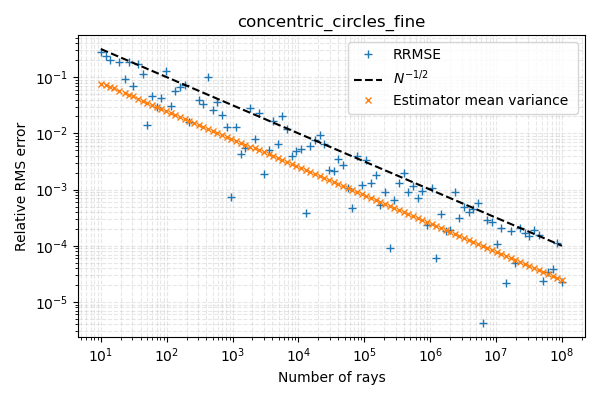
\includegraphics[width=\linewidth]{PICTURES/c2/VERIF/convergence_cc_fine.png}
\small\textbf{(b) Deux cercles concentriques}
\end{minipage}
\caption{Convergence des facteurs de vue pour deux géométries bidimensionnelles.}
\label{fig:verif2D}
\end{figure}

\subsubsection{Simulation MCRT avec des faces réfléchissantes}
\label{part:verifmiroir}

\begin{figure}[H]
\centering
\begin{minipage}{0.49\textwidth}
\centering
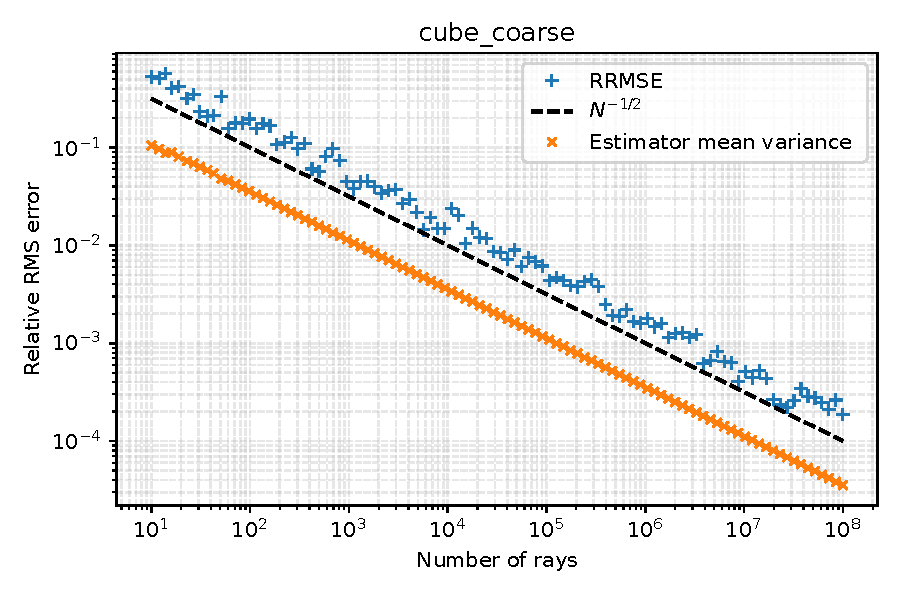
\includegraphics[width=\linewidth]{PICTURES/c2/VERIF/convergence_cube_sym_coarse.pdf}
\small\textbf{(a) Cube comportant une face réfléchissante}
\end{minipage}
\hfill
\begin{minipage}{0.49\textwidth}
\centering
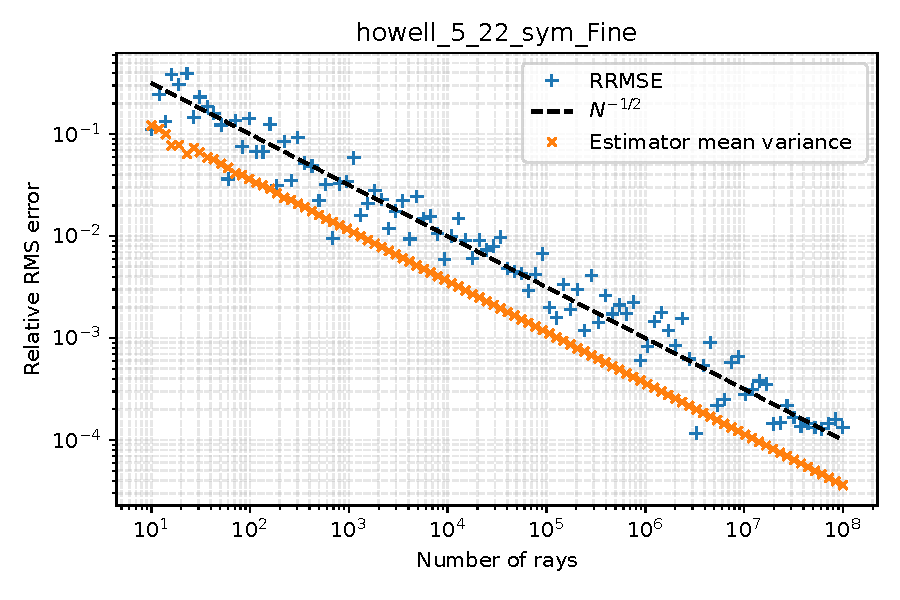
\includegraphics[width=\linewidth]{PICTURES/c2/VERIF/convergence_h5_22_sym_Fine.pdf}
\small\textbf{(b) Rangée infinie de cylindres}
\end{minipage}
\caption{Convergence des facteurs de vue pour des configurations comportant des surfaces réfléchissantes.}
\label{fig:verifmiroir}
\end{figure}

Pour les six cas de vérification des facteurs de vue présentés dans le rapport, la décroissance de la RRMSE est globalement conforme à la loi théorique en $N^{-1/2}$. Les fluctuations observées pour les faibles nombres de rayons sont caractéristiques de la variance inhérente aux méthodes de Monte Carlo et diminuent progressivement lorsque le nombre d'échantillons augmente. Dans tous les cas, la RRMSE se rapproche de la variance estimée lorsque le nombre de rayons devient suffisamment grand, ce qui indique que l'erreur est alors principalement gouvernée par les fluctuations statistiques de l'estimateur. Ces résultats montrent que l'implémentation du MCRT présente le comportement de convergence attendu et vérifie son utilisation pour le calcul des facteurs de vue sur l'ensemble des géométries considérées.



\section{Vérifications des flux radiatifs}

\subsection{Calcul des flux radiatifs}

Une fois les facteurs de vue calculés, ceux-ci sont utilisés pour déterminer les flux radiatifs échangés entre les surfaces, à partir du système de radiosités introduit en Équation~\ref{def:radio} :
$J_i = \varepsilon_i \sigma T_i^4 + (1-\varepsilon_i)\sum_{j=1}^{N} F_{ij}J_j$,
où $\varepsilon_i$ est l'émissivité de la surface $i$, $T_i$ sa température, $\sigma$ la constante de Stefan-Boltzmann et $F_{ij}$ le facteur de vue entre les surfaces $i$ et $j$.

En introduisant le vecteur des radiosités $\mathbf{J}$, le vecteur $\mathbf{T}^4$ et la matrice diagonale des émissivités $\mathbf{E}=\mathrm{diag}(\varepsilon_1,\ldots,\varepsilon_N)$, ce système se réécrit sous forme matricielle :

\begin{equation}
\left[\mathbf{I} - (\mathbf{I}-\mathbf{E})\mathbf{F}\right]\mathbf{J} = \mathbf{E}\sigma\mathbf{T}^4.
\label{eq:systeme_radiosite}
\end{equation}

La matrice $\mathbf{A} = \mathbf{I} - (\mathbf{I}-\mathbf{E})\mathbf{F}$, construite à partir des facteurs de vue et des émissivités, permet ainsi de résoudre ce système linéaire pour obtenir les radiosités de l'ensemble des surfaces. Le flux radiatif net quittant chaque surface s'en déduit par $q_i = J_i - \sum_{j=1}^{N} F_{ij}J_j$, soit sous forme matricielle $\mathbf{q} = (\mathbf{I}-\mathbf{F})\mathbf{J}$, ce qui conduit à l'expression finale :

\begin{equation}
\mathbf{q} = (\mathbf{I}-\mathbf{F})\left[\mathbf{I} - (\mathbf{I}-\mathbf{E})\mathbf{F}\right]^{-1} \mathbf{E}\sigma\mathbf{T}^4.
\label{eq:q_final}
\end{equation}
\subsection{Vérification du calcul des flux radiatifs}

La méthode de calcul des flux radiatifs a été vérifiée à partir de deux cas de référence issus de \cite{howell}, permettant de vérifier l'utilisation des facteurs de vue calculés par le MCRT dans la résolution des échanges radiatifs entre surfaces diffuses grises. Dans les deux cas, aucune méthode de correction des facteurs de vue (Section~\ref{part:renforcement}) n'a été appliquée : les facteurs de vue utilisés sont directement ceux issus de l'estimation Monte Carlo brute, avec un écart-type maximal de $10^{-3}$ ($10^6$ rayons) sur les coefficients de la matrice $F$.

\subsubsection{Deux cylindres concentriques infinis}

Le premier cas correspond à l'exemple 5.5 de \cite{howell} : deux cylindres concentriques infinis, le cylindre extérieur étant divisé en deux demi-cylindres maintenus à des températures différentes, avec $T_{\mathrm{int}}=1700$~K, $T_{\mathrm{ext},1}=1207$~K et $T_{\mathrm{ext},2}=1415$~K.

\begin{table}[H]
\centering
\begin{tabular}{lc}
\toprule
Surface & Flux radiatif (W.m$^{-2}$) \\
\midrule
Cylindre intérieur & $2.9976\times10^{5}$ \\
Demi-cylindre extérieur 1 & $-1.9994\times10^{5}$ \\
Demi-cylindre extérieur 2 & $-9.9792\times10^{4}$ \\
\bottomrule
\end{tabular}
\caption{Flux radiatifs obtenus pour l'exemple 5.5 de \cite{howell}.}
\label{tab:flux_howell55}
\end{table}

Les flux obtenus sont en accord, aux deux chiffres significatifs près, avec la solution de référence de \cite{howell}, dont la précision se limite à deux chiffres significatifs. Cet accord, obtenu sans correction des facteurs de vue, illustre leur bonne convergence statistique pour ce niveau d'échantillonnage. Le bilan énergétique est par ailleurs vérifié avec une erreur inférieure à $10^{-4}$~W.m$^{-2}$.

\subsubsection{Pastille combustible dans une cavité carrée}

Le second cas correspond à l'exercice 5.22 de \cite{howell} : une pastille cylindrique placée au centre d'une cavité carrée, dont trois parois sont maintenues à température nulle, les surfaces rayonnantes ayant une émissivité de 0,5. Les températures imposées sont $T_{\mathrm{fuel}}=1000$~K et $T_{\mathrm{parois}}=674, 0, 0, 0$~K. Le flux radiatif calculé pour la pastille est $q_{\mathrm{fuel}} = 8.4473\times10^{4}$~W.m$^{-1}$, en accord avec la valeur de référence de \cite{howell}. Comme pour le cas précédent, cet accord confirme la bonne convergence statistique des facteurs de vue bruts utilisés. Les flux nets satisfont également le bilan énergétique, avec un écart sur la fermeture du système inférieur à $10^{-4}$~W.m$^{-1}$.

Ces deux cas montrent ainsi que la résolution du système de radiosités permet de retrouver les flux radiatifs de référence à partir des facteurs de vue bruts calculés par le MCRT, sans recours à une correction, tout en respectant la conservation de l'énergie.